\section{Results and Analysis}

\subsection{RQ1: Generalisation of FOLtR-ES performance beyond MQ2007/2008}
For answering RQ1 we replicate the results obtained by Kharitonov~\cite{kharitonov2019federated} on the MQ2007 and MQ2008 datasets; we then reproduce the experiment on MSLR-WEB10k and Yahoo datasets, on which FOLtR-ES has not been yet investigated, and we compare the findings across datasets. For these experiments we use antithetic variates, set the number of interactions $B = 4$ and simulate 2,000 clients, use MaxRR as reward signal and for evaluation on clicked items. 

\begin{figure}[t]
	\centering
	\begin{subfigure}{1\textwidth}
		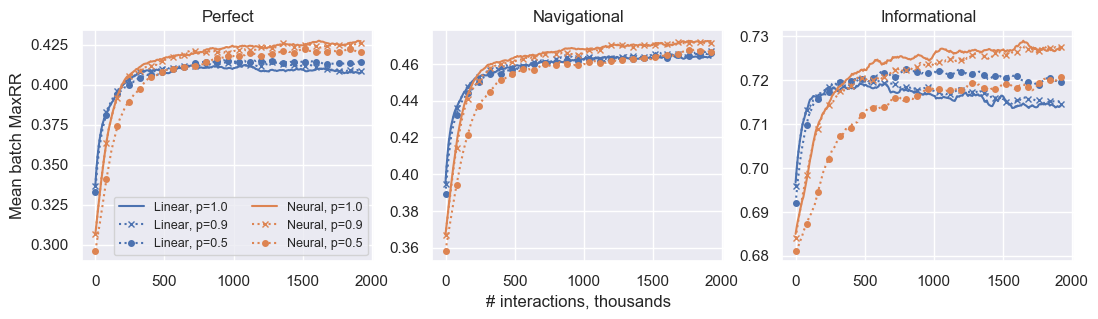
\includegraphics[width=13cm, height=3.5cm]{images/RQ1/mq2007_foltr_c2000_ps.png}
		\caption{Mean batch MaxRR for MQ2007.}
		\label{fig:mq2007-rq1}
	\end{subfigure}
	\begin{subfigure}{1\textwidth}
		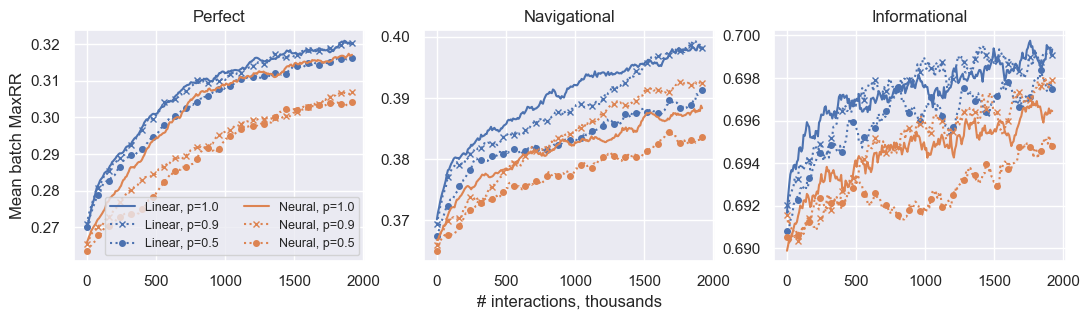
\includegraphics[width=13cm, height=3.5cm]{images/RQ1/mslr10k_foltr_c2000_ps.png}
		\caption{Mean batch MaxRR for MSLR-WEB10k.}
		\label{fig:mslr10k-rq1}
	\end{subfigure}
	\begin{subfigure}{1\textwidth}
		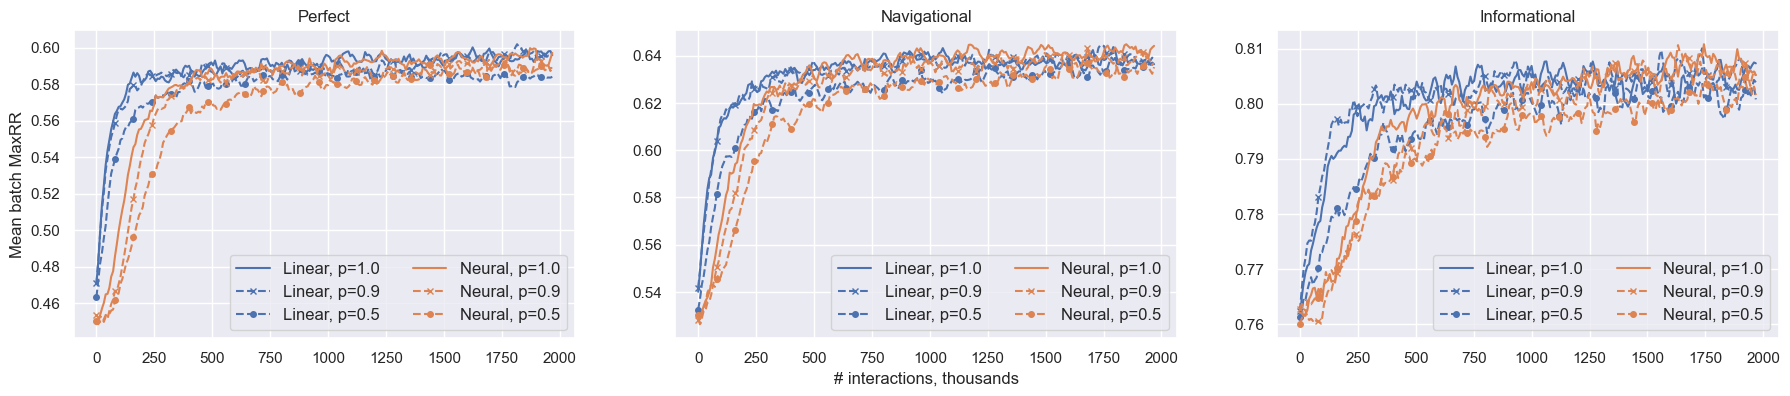
\includegraphics[width=13cm, height=3.5cm]{images/RQ1/yahoo_foltr_c2000_ps.png}
		\caption{Mean batch MaxRR for Yahoo!.}
		\label{fig:yahoo-rq1}
	\end{subfigure}
	\caption{{\color{red}{Results for RQ1: performance of FOLtR-ES across datasets under three different click models (averaged across all dataset splits).}} \label{fig:RQ1}}
\end{figure}

Figure~\ref{fig:mq2007-rq1} reports the results obtained by FOLtR-ES on the MQ2007 dataset\footnote{Similar results were obtained for MQ2008 and are omitted for space reasons.} with respect to the three click models considered, various settings for the privatization parameter $p$, and the two FOLtR-ES methods (linear and neural). Our results fully replicate those of Kharitonov~\cite{kharitonov2019federated} and indicate the following findings: (1) FOLtR-ES allows for the iterative learning of effective rankers; (2) high values of $p$ (lesser privacy) provide higher effectiveness; 
(3) the neural ranker is more effective than the linear ranker when $p \rightarrow 1$ (small to no privacy), while the linear model is equivalent, or better (for informational clicks) when $p=0.5$. 

However, not all these findings are applicable to the results obtained when considering MSLR-WEB10k and Yahoo!, which are displayed in Figures~\ref{fig:mslr10k-rq1} and~\ref{fig:yahoo-rq1}. In particular, we observe that (1) the results for MSLR-WEB10k (and to a lesser extent also for Yahoo!) obtained with the informational click model are very unstable, and, regardless of the click model, FOLtR-ES requires more data than with MQ2007/2008 to arrive at a stable performance, when it does; (2) the neural ranker is less effective than the linear ranker, especially on MSLR-WEB10k. We believe these findings are due to the fact that query-document pairs in MSLR-WEB10k and Yahoo! are represented by a larger number of features than in MQ2007/2008. Thus, more data is required for effective training, especially for the neural model; we also note that FOLtR-ES is largely affected by noisy clicks in MSLR-WEB10k. 

\subsection{RQ2: Effect of number of clients on FOLtR-ES}
To answer RQ2 we vary the number of clients involved in FOLtR-ES; we investigate the values \{50, 1,000, 2,000\}. Kharitonov~\cite{kharitonov2019federated} used 2,000 in the original experiments, and the impact of the number {\color{red}{has not been studied}}. To be able to fairly compare results across number of clients, we fixed the total number of ranker updates to 2,000,000; we also set $B = 4$ and $p=0.9$. We perform these experiments on all three datasets considered in this paper, but we omit to report results for Yahoo! due to space limitations. 

\begin{figure}[t]
	\centering
	\begin{subfigure}{1\textwidth}
		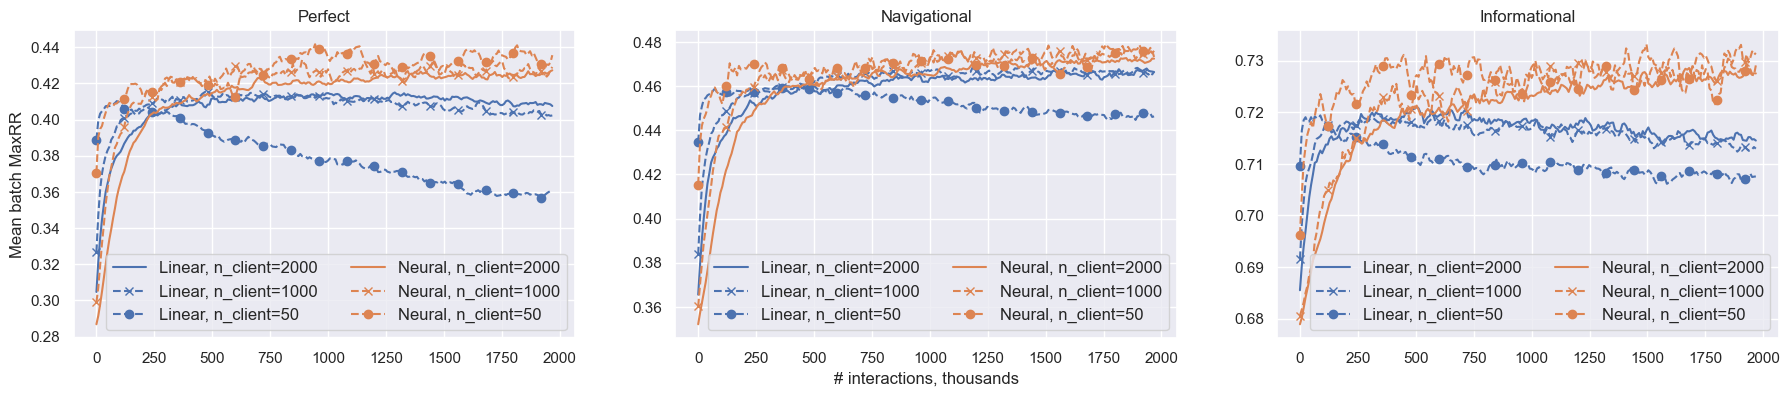
\includegraphics[width=13cm, height=3.5cm]{images/RQ2/mq2007_foltr_client_both_p0.9.png}
		\caption{Mean batch MaxRR for MQ2007.}
		\label{fig:mq2007-rq2}
	\end{subfigure}
	\begin{subfigure}{1\textwidth}
		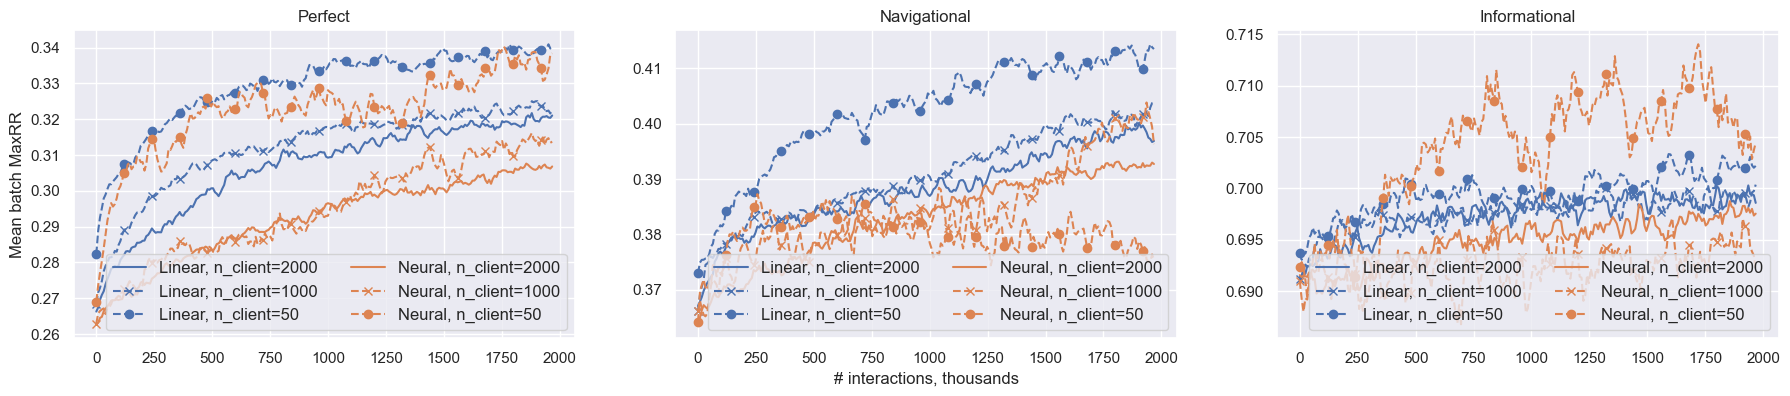
\includegraphics[width=13cm, height=3.5cm]{images/RQ2/mslr10k_foltr_client_both_p0.9.png}
		\caption{Mean batch MaxRR for MSLR-WEB10k.}
		\label{fig:mslr10k-rq2}
	\end{subfigure}
	\caption{{\color{red}{Results for RQ2: performance of FOLtR-ES with respect to number of clients (averaged across all dataset splits).}} \label{fig:RQ2}} 
\end{figure}

The results of these experiments are reported in Figure~\ref{fig:RQ2}, and they are mixed. For MQ2007, the number of clients have little effect on the neural ranker used in FOLtR-ES, although when informational clicks are provided this ranker is less stable, although often more effective, if very few clients (50) are used. Having just 50 clients, instead, severally hits the performance of the linear ranker, when compared with 1,000 or 2,000 clients. The findings on MSLR-WEB10k, however, are different. In this dataset, a smaller number of clients (50), is generally better than larger numbers, both for linear and neural ranker. An exception to this is when considering navigational clicks: in this case the linear ranker obtains by far the best performance with a small number of clients, but the neural ranker obtains the worst performance. This suggest that the number of clients greatly affects FOLtR-ES: but trends are not consistent across click types and datasets. 

\subsection{RQ3: Comparing FOLtR-ES to state-of-the-art OLTR methods}
The original study of FOLtR-ES did not compared the method with non-federated OLTR approaches. To contextualise the performance of FOLtR-ES and to understand the trade-off between privacy and performance when designing FOLtR-ES, we compare this method with the current state-of-the-art OLTR method, the Pairwise Differentiable Gradient Descent (PDGD)~\cite{oosterhuis2018differentiable}. For fair comparison, we set the privatization parameter $p=1$ (lowest privacy) and the number of clients to 2,000. In addition note that in normal OLTR settings, rankers are updated after each user interaction: however in FOLtR-ES, rankers are updated in small batches. For fair comparison, we adapt PDGD to be updated in batch too. Instead of updating the ranker after each interaction (batch size 1), we accumulate gradients computed on the same batch size as for FOLtR-ES. Specifically, with 2000 clients for FOLtR-ES, the batch size of each update is 8,000 iterations (4 $\times$ 2,000). We then compute the updated gradients for PDGD on 8,000 interactions too. %Note, the number of updates after 2m user interaction now becomes 2m/8000 = 250.
We perform these experiments on all three datasets considered in this paper, but we omit to report results for Yahoo! due to space limitations. 

\begin{figure}[t]
	\centering
	\begin{subfigure}{1\textwidth}
		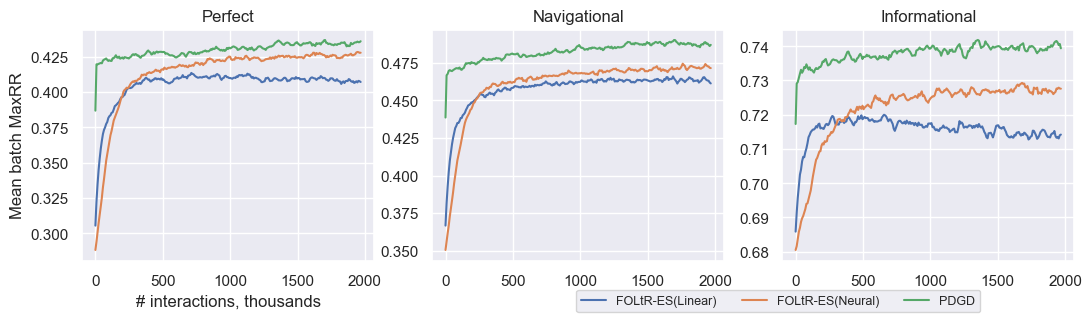
\includegraphics[width=13cm, height=3.5cm]{images/RQ3/mq2007_foltr_PDGD_mrr_c2000_p1.0.png}
		\caption{Mean batch MaxRR for MQ2007.}
		\label{fig:mq2007-rq3}
	\end{subfigure}
	\begin{subfigure}{1\textwidth}
		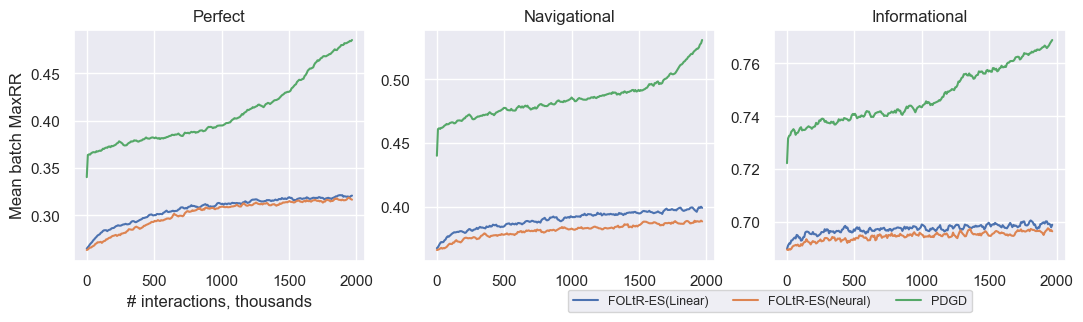
\includegraphics[width=13cm, height=3.5cm]{images/RQ3/mslr10k_foltr_PDGD_mrr_c2000_p1.0.png}
		\caption{Mean batch MaxRR for MSLR-WEB10k}
		\label{fig:mslr10k-rq3}
	\end{subfigure}
	\caption{{\color{red}{Results for RQ3: performance of FOLtR-ES and PDGD across datasets with privatization parameter $p=1$ and 2,000 clients (averaged across all dataset splits).}} \label{fig:RQ3}} 
\end{figure}

Results are shown in Figure~\ref{fig:RQ3}: regardless of linear or neural ranker, FOLtR-ES is less effective than PDGD. The gap in performance is greater in larger datasets like MSLR-WEB10k than in the smaller MQ2007/2008. This gap becomes even bigger, especially for the first iterations, if the PDGD ranker was updated after each iteration (not shown here), rather than after a batch has been completed. This highlights that FOLtR-ES has the merit of being the first privacy preserving federated OLTR approach available; however, more work is needed to improve the performance of FOLtR based methods so as to close the gap between privacy-oriented approaches and centralise approaches that do not consider user privacy.

\subsection{RQ4: Extending FOLtR-ES evaluation to common OLTR practice}
In the original work and in the sections above, FOLtR-ES was evaluated using MaxRR computed with respect to the clicks performed by the simulated users (click models). This is an unusual evaluation for OLTR because: (1) usually nDCG@10 is used in place of MaxRR as metric, (2) nDCG is computed with respect to relevance labels, and not clicks, and on a withheld portion of the dataset, not on the interactions observed -- this is used to produce learning curves and is referred to as offline nDCG, (3) in addition online nDCG is measured from the relevance labels in the SERPs from which clicks are obtained, and either displayed as learning curves or accumulated throughout the sessions -- these values represent how OLTR has affected user experience. We then consider this more common evaluation of OLTR next, where we set the number of clients to 2,000 and experiment with $p=\{0.5, 0.9, 1.0\}$; we omit to report results for Yahoo! due to space limitations. 

\begin{figure}[t]
	\centering
	\begin{subfigure}{1\textwidth}
		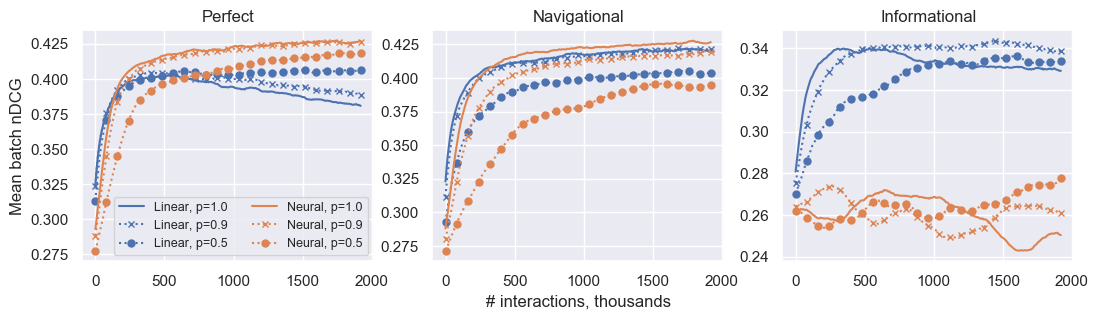
\includegraphics[width=13cm, height=3.5cm]{images/RQ4/mq2007_foltr_online nDCG_both_c2000_ps.png}
		\caption{Mean batch nDCG@10 for MQ2007.}
		\label{fig:mq2007-rq4}
	\end{subfigure}
	\begin{subfigure}{1\textwidth}
		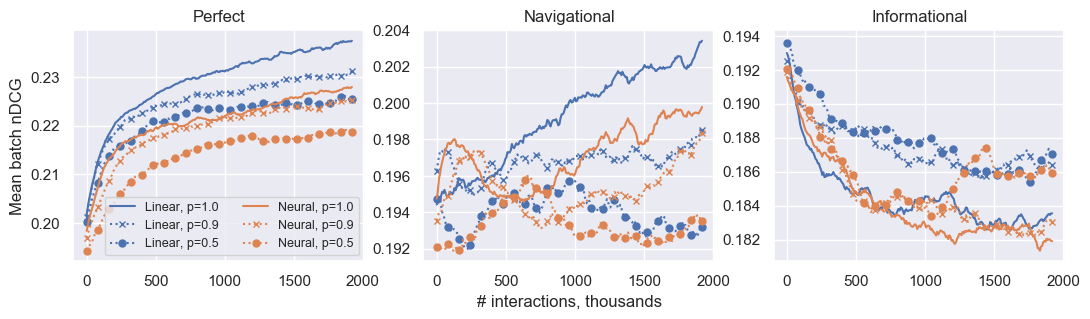
\includegraphics[width=13cm, height=3.5cm]{images/RQ4/mslr10k_foltr_online nDCG_both_c2000_ps.png}
		\caption{Mean batch nDCG@10 for MSLR-WEB10k.}
		\label{fig:mslr10k-rq4}
	\end{subfigure}
	\caption{{\color{red}{Results for RQ4: performance of FOLtR-ES in terms of online nDCG@10 computed using relevance labels and the SERPs used for obtaining user iterations (averaged across all dataset splits).}} \label{fig:RQ4}} 
\end{figure}

\begin{figure}[t]
	\centering
	\begin{subfigure}{1\textwidth}
		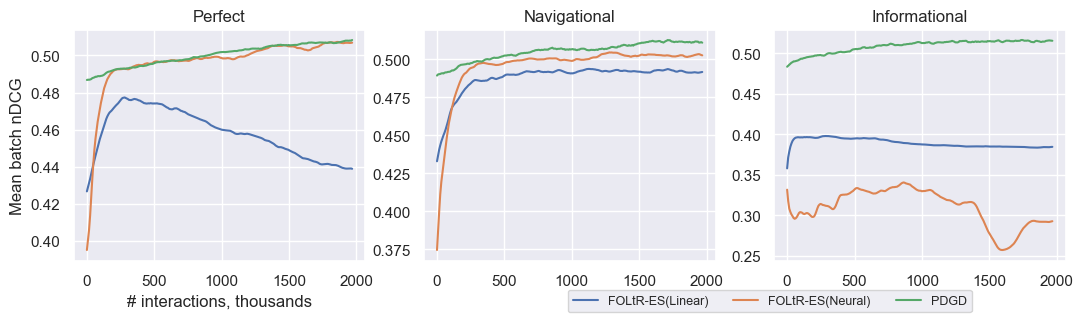
\includegraphics[width=13cm, height=3.5cm]{images/RQ4/mq2007_foltr_PDGD_offline nDCG_c2000_p1.0.png}
		\caption{Mean batch nDCG@10 for MQ2007.}
		\label{fig:mq2007-rq4-offline}
	\end{subfigure}
	\begin{subfigure}{1\textwidth}
		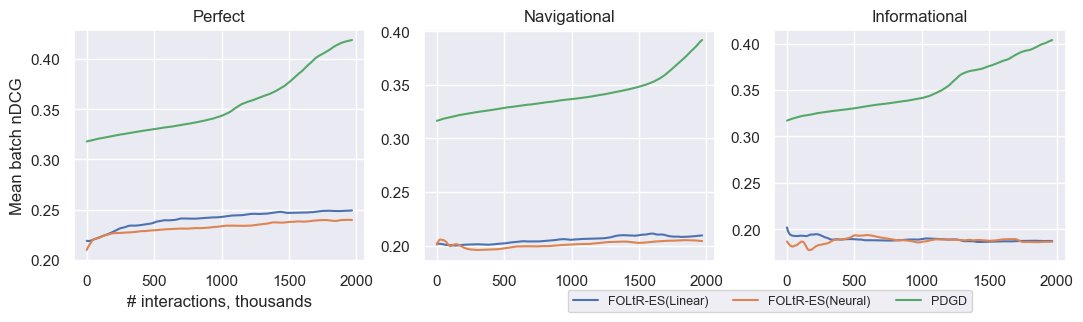
\includegraphics[width=13cm, height=3.5cm]{images/RQ4/mslr10k_foltr_PDGD_offline nDCG_c2000_p1.0.png}
		\caption{Mean batch nDCG@10 for MSLR-WEB10k.}
		\label{fig:mslr10k-rq4-offline}
	\end{subfigure}
	\caption{{\color{red}{Results for RQ4: performance of FOLtR-ES and PDGD in terms of offline nDCG@10 with privatization parameter $p=1$ and 2,000 clients (averaged across all dataset splits).}} \label{fig:RQ4-offline}} 
\end{figure}

Results are reported in Figure~\ref{fig:RQ4}. It is interesting to compare these plots with those in Figure~\ref{fig:RQ1}, that relate to the unusual (for OLTR) evaluation setting used in the original FOLtR-ES work. By comparing the figures, we note that for MQ2007, FOLtR-ES can effectively learn rankers for perfect and navigational clicks. However, when the clicks become noisier (informational clicks), then FOLtR-ES learning is effective for the linear ranker but no learning occurs for the neural ranker: this is unlikely in the evaluation settings of the original work (Figure~\ref{fig:RQ1}). We note this finding repeating also for MSLR-WEB10k, but this time this affects both linear and neural rankers; we also note that the online performance in MSLR-WEB10k on navigational clicks are also quite unstable and exhibit little learning for specific values of $p$ and ranker type. {\color{red}{The online performance in MSLR10k on informational clicks (the noisiest clicks) even shows a decreasing trend as the update grows.}}

We further investigate the performance of FOLtR-ES with respect to offline nDCG@10. Results are shown in Figure~\ref{fig:RQ4-offline}, and are plotted along with the offline nDCG@10 of PDGD for additional context. Also the offline performance confirm that FOLtR-ES does not provide stable learning across click settings, datasets and ranker types. We also note that the performance of PDGD are sensibly higher than that of FOLtR-ES, apart for the neural ranker on MQ2007 when perfect and navigational clicks are considered. 

These findings suggest that FOLtR-ES is yet far from being a solution that can be considered for use in practice, and more research is required for devising effective federated, privacy-aware OLTR techniques.